\chapter{從波動認識物理}
\chapterauthor{丁安磊}

\section{一進一出:函數專論}

\subsection{為什麼?}

數學家發明了函數,為了討論兩種\textbf{變數}之間的\textbf{關係},而在物理的研究過程中,也常需要討論各個\textbf{物理量}之間的\textbf{關係}(物理量是變數的一種),函數是兩種變數之間的對應關係,大致概念如下圖所示。

\begin{figure}[H]
\centering
\graphicspath{{physics/}}
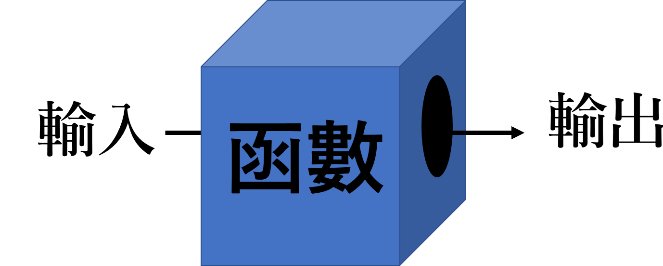
\includegraphics[width=5cm, center]{blackox.png}
\caption{把函數比喻成箱子,會將輸入的變數轉化為輸出的變數。} \vskip 10 pt
\label{fig:blackbox}
\end{figure}
\subsection{函數的呈現}

我們可以有許多方法呈現這這個箱子到底做了甚麼,以下列舉幾種。

\begin{enumerate}
	\item \textbf{文字:}
	\begin{enumerate}
		\item 圓面積與半徑的平方成正比
		\item 密度與質量成正比、與體積成反比
		\item 當體積固定密度與質量成正比
	\end{enumerate}
	\item \textbf{函數圖表:} \\
		例如: \\
		\begin{table}[H]
		\centering
		\begin{tabular}{|c|c|}
		\hline
		\textbf{正多邊形}      & \textbf{內角角度}  	    \\ \hline
		正三角形      & $60^\circ$    \\ \hline
		正四邊形      & $90^\circ$    \\ \hline
		正五邊形      & $108^\circ$    \\ \hline
		正六邊形      & $120^\circ$    \\ \hline
         $\vdots $ &  $\vdots $     \\ \hline
		你爽的話可以繼續寫 & 可是我好懶 \\ \hline
	
		\end{tabular}
		\end{table}
	\item \textbf{函數圖形:}\\
當我們劃出圖形的表格,我們能夠把他標示在有由$x$軸和$y$軸形成的平面上。以$y=x^2$為例,一開始我們計算$x$和$y$的幾個對應關係,把它畫在平面上,接著越算越多,我們就能預測並畫出$y=x^2$的圖形。
\begin{figure}[H]
\centering
\graphicspath{{physics/}}
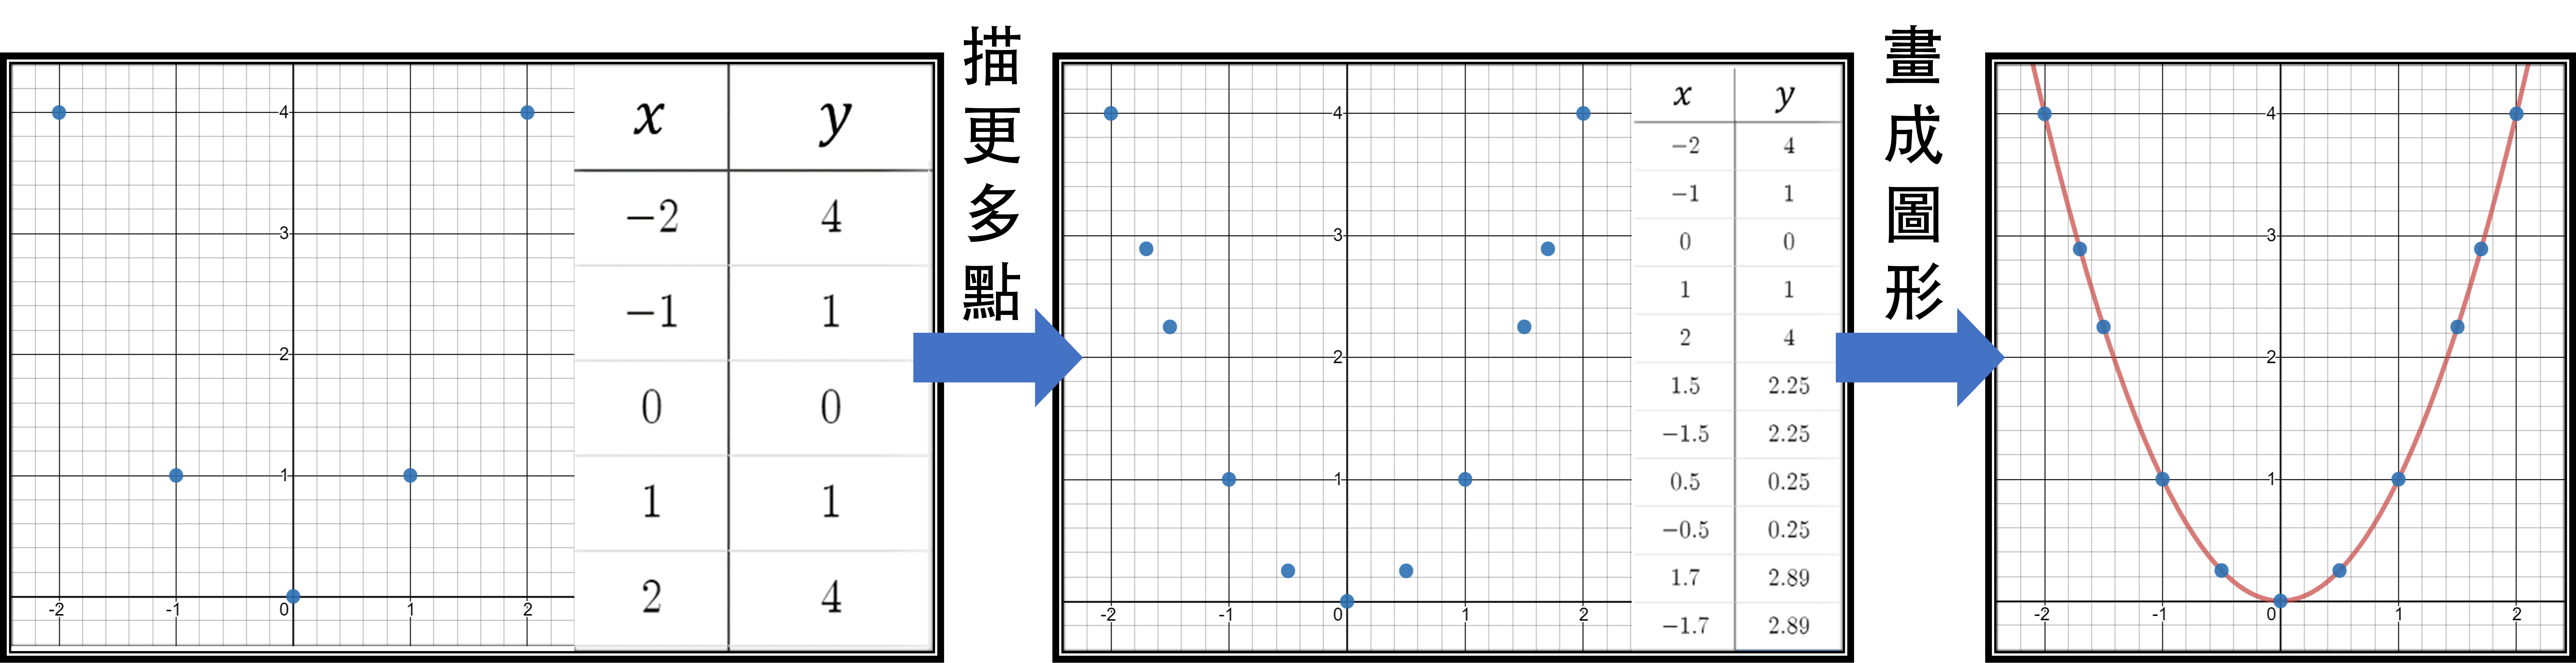
\includegraphics[width=\textwidth, center]{function_graph.png}
\label{fig:function1}
\end{figure}

	\item \textbf{數學式:} \\
這裡就舉幾個數學和物理常用到的公式來理解吧。
		\begin{figure}[H]
		\centering
		\graphicspath{{physics/}}
		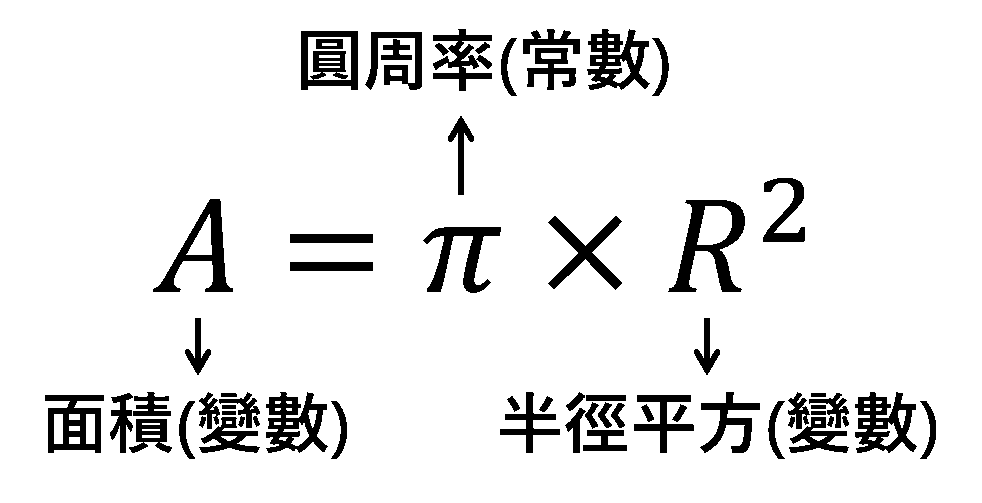
\includegraphics[width=5cm, center]{A.png}
		\caption{$A=f(R)$} \vskip 10 pt
		\label{fig:A}
		\end{figure}
				
		\begin{figure}[H]
		\centering
		\graphicspath{{physics/}}
		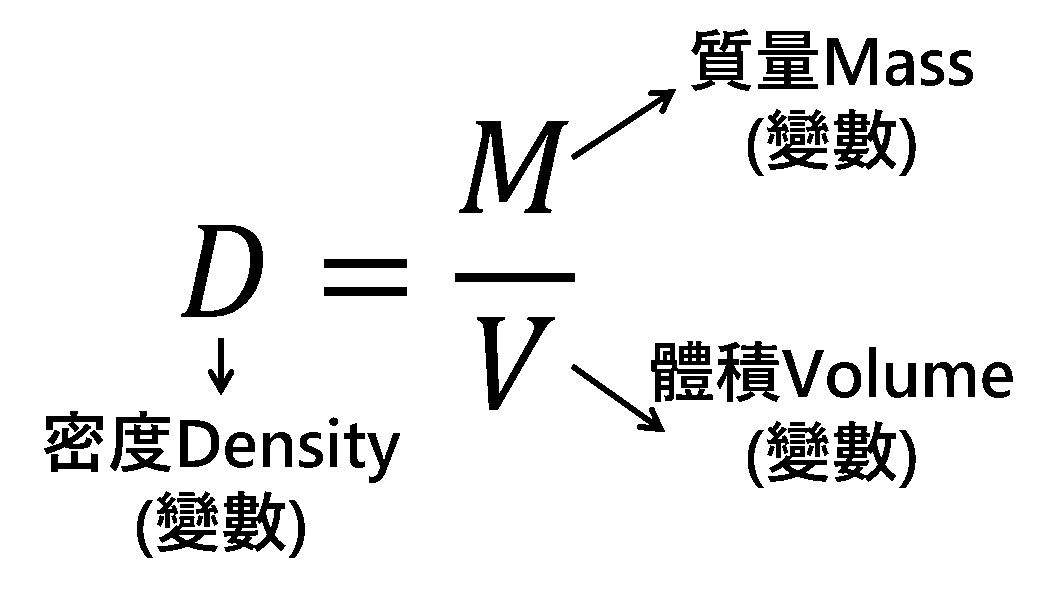
\includegraphics[width=5cm, center]{D1.png}
		\caption{$D=f(V,M)$} \vskip 10 pt
		\label{fig:D1}
		\end{figure}
		
		\begin{figure}[H]
		\centering
		\graphicspath{{physics/}}
		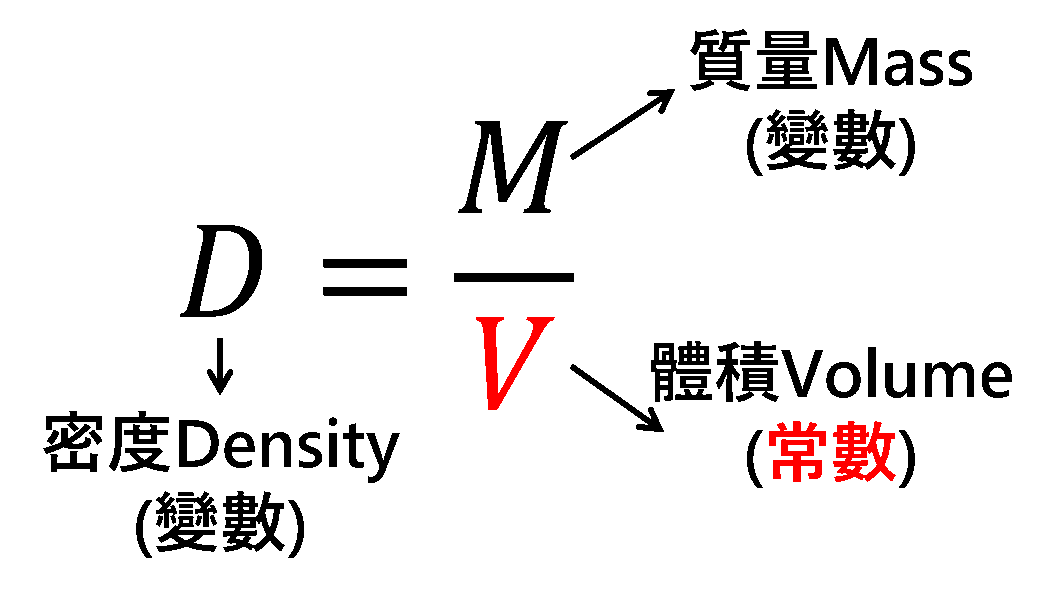
\includegraphics[width=5cm, center]{D2.png}
		\caption{$D=f(M)$} \vskip 10 pt
		\label{fig:D2}
		\end{figure}
\end{enumerate}

\section{聽起來很厲害:三角函數}
\subsection{複習:直角三角形的三角函數}
\begin{figure}[H]
\centering
\graphicspath{{physics/}}
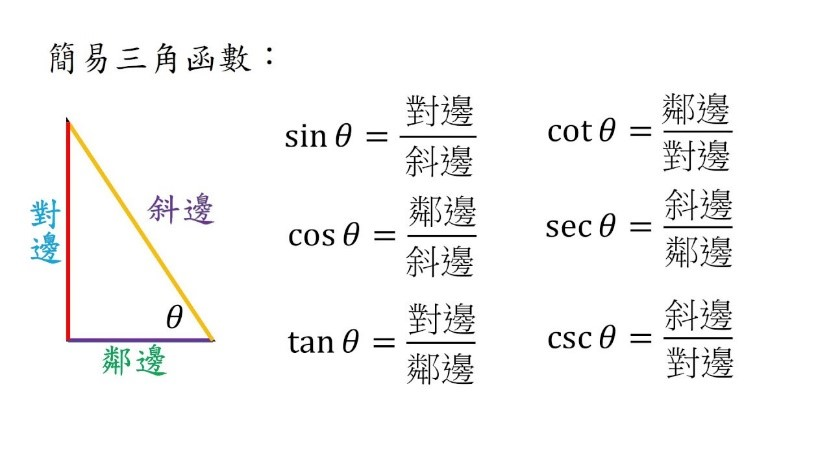
\includegraphics[width=7.5cm, center]{tri-function.jpg}
\caption{簡易三角函數} \vskip 10 pt
\label{fig:tri-function}
\end{figure}
\subsection{角的度量、換算與方向:}
\subsubsection{度($360^\circ$制)}
相信大家學過360°是什麼意思了,那為什麼要用360這個數字呢?因為古巴比倫人是用60進位,然後地球公轉差不多花360多天,這樣每天太陽差不多動一度,還有如果不是用360這種漂亮的數字的話,上面的正多邊形內角的表的數字就會很醜,我就不想打講義了。
\subsubsection{弧度(弳度制)}
在物理上,我們多使用弧度來度量角,弧度的定義如下:

\begin{center}
{\Kai 在圓周上,截取與半徑等長之弧,則此弧所對的圓心角稱為一弧度(或稱為一弳)} 
\end{center}

\noindent
因為科學家都很懶,以弧度為單位表示會省略單位。\\
所以我們看到角有度就是度,看到沒度就是弧度(?\\

\subsubsection{換算}
又因為單位圓的周長為$2\pi$,所以$360^\circ=2\pi$由此可得$1=(360^\circ )/2\pi \approx 57.29^\circ$,且$1^\circ=\frac{2\pi}{360^\circ}=0.0174533$。
\begin{figure}[H]
\centering
\graphicspath{{physics/}}
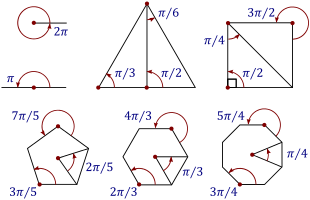
\includegraphics[width=7.5cm, center]{num-shape.png}
\caption{可以自己驗證看看} \vskip 10 pt
\label{fig:num-shape}
\end{figure}
\subsubsection{有向角}
以前我們學的角度不討論方向,但為了後面的廣義三角函數,我們定義角度的方向逆時針。
至於為什麼角度要這樣定義呢,等等就知道。 

所以一條線(始邊)繞著一個點旋轉後,變成另一條線(終邊),如果他逆時針轉,角度為正值,反之則為負值。

\begin{figure}[H]
\centering
\graphicspath{{physics/}}
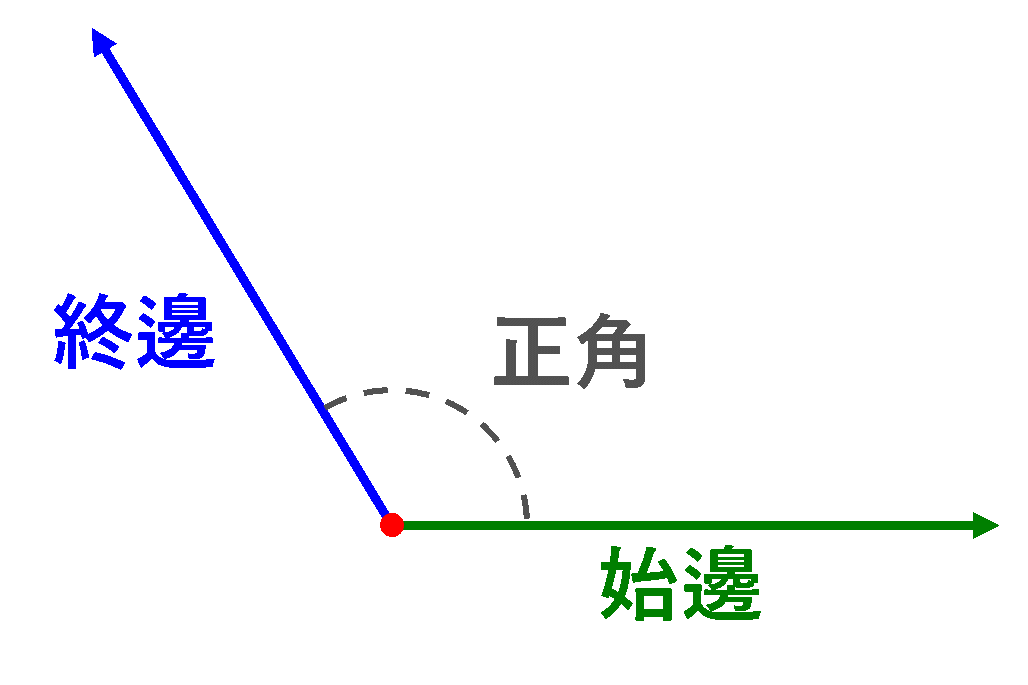
\includegraphics[width=7.5cm, center]{pos-angle.png}
\caption{正角} \vskip 10 pt
\label{fig:pos-angle}
\end{figure}

\begin{figure}[H]
\centering
\graphicspath{{physics/}}
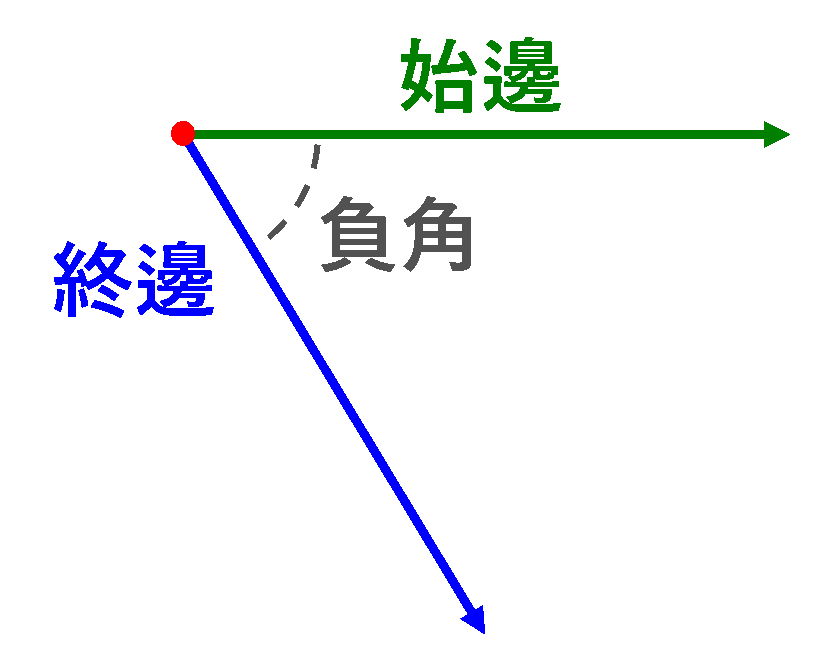
\includegraphics[width=7.5cm, center]{neg-angle.png}
\caption{負角} \vskip 10 pt
\label{fig:neg-angle}
\end{figure}

\noindent
\fbox{小測驗}
\begin{enumerate}
\item 這張圖中的廣義角是多少?
\begin{figure}[H]
\centering
\graphicspath{{physics/}}
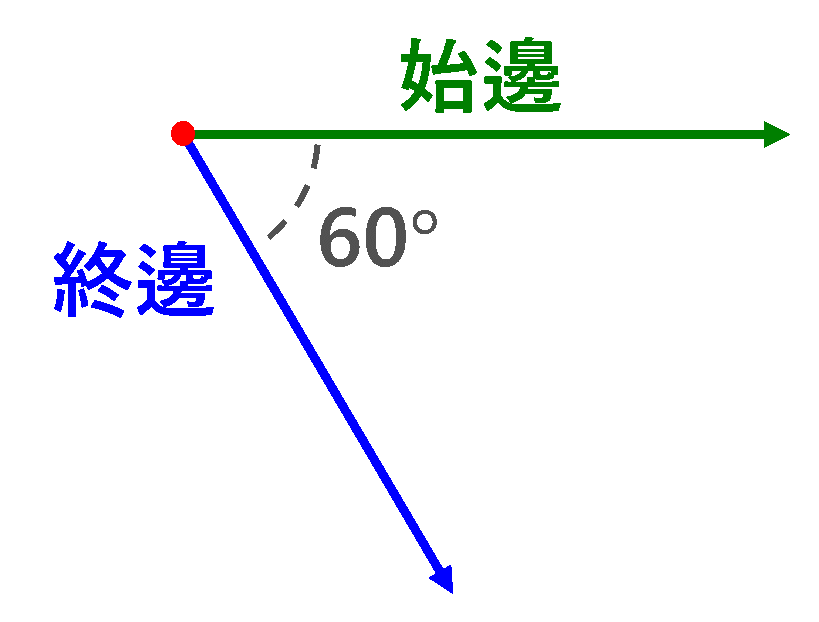
\includegraphics[width=7.5cm, center]{angle-test.png}
\label{fig:angle-test}
\end{figure}
\item 過了兩天,時鐘上的時針分針秒針轉了多少?
\end{enumerate}

\subsubsection{廣義三角函數}
在討論簡易三角函數的時候,我們無論如何都不能超過$90^\circ$
\begin{figure}[H]
\centering
\graphicspath{{physics/}}
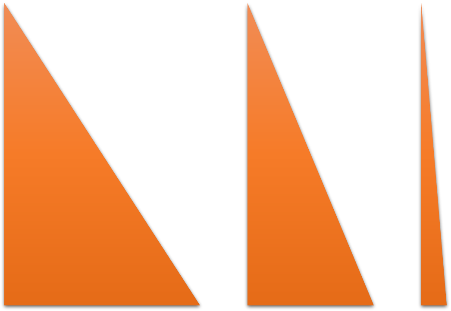
\includegraphics[width=7.5cm, center]{over-90-tri.png}
\caption{怎麼壓都不會超過$90^\circ$} \vskip 10 pt
\label{fig:neg-angle}
\end{figure}

於是數學家為了推廣,使用單位圓定義三角函數
\begin{center}
\begin{equation*}
   \addtolength{\fboxsep}{5pt}
    \boxed{
    \begin{gathered}
   		\mbox{單位圓(半徑為1)上的一點,繞轉了}\theta \mbox{時,} \\
   		\mbox{使用此點的x,y座標定義三角函數:} \\
		x=\cos \theta \\
		y=\sin \theta 
    \end{gathered}
    }
\end{equation*}
\end{center}

這樣做的話,$\theta$在$0^\circ \sim 90^\circ$的範圍內,保持和簡易三角函數一樣,又能突破原本的限制。

\begin{figure}[H]
\centering
\graphicspath{{physics/}}
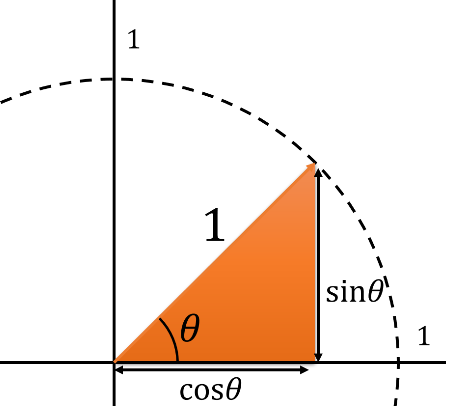
\includegraphics[width=7.5cm, center]{broad-tri-function.png}
\caption{廣義三角函數} \vskip 10 pt
\label{fig:broad-tri-function}
\end{figure}

\noindent
\fbox{小測驗}
\begin{enumerate}
\item $\sin (120^\circ)=$?,$\sin (\frac{2}{3} \pi)=$?
\item $\sin (\theta) = \frac{1}{2}$,$\theta =$?
\end{enumerate}

\subsection{三角函數的度量}
我們剛剛推廣了三角函數,本來我們的三角函數只能吃$0$到$\frac{\pi}{2}$之間的角度,但推廣之後任何數都可以是三角函數的輸入值,所以可以畫出函數的關係圖,六種三角函數都可以畫圖,不過我們先來關心最基本的:$\sin$函數圖(正弦函數圖)\\

要如何畫出$\sin$函數圖呢?課本裡通常使用無聊的描點法,不過這堂課已經夠無聊了,所以用投影的方法來想。

\begin{figure}[H]
\centering
\graphicspath{{physics/}}
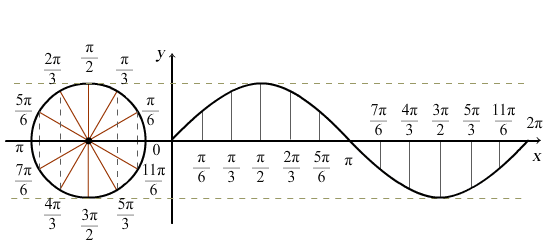
\includegraphics[width=\textwidth, center]{sin-wave.png}
\caption{$y=\sin (x)$} \vskip 10 pt
\label{fig:sin-wave}
\end{figure}

這是$y=\sin⁡ (x)$的圖畫出來的樣子,圖片是靜態的所以看起來很難,附錄裡有簡報檔案的網址可以慢慢看裡面的動畫。因為圓上的點繞了一圈會回到原點,所以後面的圖是無限重複的,我們稱$\sin$函數具有週期性,其週期為$2\pi$。

這個函數看起來很像波。事實上,在物理學,正弦波是最基本的一種波。

\section{波的計算方法}

\subsection{國中的波公式}
$$v=\frac{\lambda}{T}=\lambda f$$
\begin{center}
($v$;波速;$\lambda$:波長;$T$:週期;$f$:頻率)
\end{center}
\subsection{更BANG的波公式}
\subsubsection{簡介}
國中的波公式只能描述波速、波長、週期、頻率之間的關係,物理學家當然不會滿足,所以我們必須學習更高階的公式來描述波。

我們能夠最直接看到的就是波的偏移,以繩波為例,繩波是透過繩子作為介質傳遞的(廢話),如果我們在繩子上一點綁了一個紅色的結,如果繩子的波源例如拉繩子的手,只有上下移動,沒有左右移動,從旁邊看這個紅色的結只會上下移動,也就是說,只有波形會傳遞,介質只會上下震動並不會傳遞。

再舉一個例子聲波是空氣分子震動產生的,你可以想像敲鑼打鼓等等樂器的演奏,敲這些樂器你會讓他開始震動,於是他就會壓縮、然後放鬆(?)空氣分子,然後他的偏移(壓縮的幅度)如果越大則聲音傳到我們耳朵裡就會聽起來會越大聲

\subsubsection{與時間無關的偏移函數}
以下開始討論波的偏移與其他物理量的關係,一樣以最簡單的繩波為例,當波源製造出了正弦的繩波,按下時間暫停器,這個時候波的偏移和什麼物理量有關係?當然,是位置,不同位置的偏移量不同,所以我們可以把它們的函數這樣寫。

$$y=A \times \sin (x) \mbox{(振幅為A的正弦波)}$$
\begin{center}
($y$:偏移量;$x$:到波源的距離)
\end{center}


首先從$A$說起,在定義正弦函數的時候,我們是用單位圓,所以他會在1到-1之間震盪,但繩波的震幅不一定是1公尺,所以乘上一個$A$,稱為振幅,乘上$A$之後,繩波變成在$A\sim -A$之間震盪。


再來是$k$,同樣的,因為使用單位圓定義,所以正弦波的波長原本是$2\pi$,即一圈的角度,但繩波的波長不一定是$2\pi$公尺,所以我們要對正弦波進行拉伸,把他的波長伸長或縮短成$\lambda$。

那麼$k$要是多少才能有讓波長變成$\lambda$呢?也就是說$k$和$\lambda$的關係是什麼?

我們剛剛知道,$\sin$裡面包的是指一個角度,我們稱為\textbf{相角},所以對這個函數來說,$\sin$裡面包的是$kx$,我們把他當成單位圓上某點的的角度,當$x$逐漸增大,$kx$這個相角也開始改變,而且如果我們已知這個波的波長為$\lambda$,所以當$x$從0慢慢增加到$\lambda$的時候,$kx$也剛好走了一圈($2\pi$),所以會有

$$
k \times \lambda-k \times 0=2 \pi
$$

所以
$$ k = \frac{2\pi}{\lambda} $$

於是我們就推出來$k$與$\lambda$的關係,你可能會發現,我特別把$k\times0$這一項標出來,為什麼呢?因為你的起點可以任意決定。
比方說,對跟剛剛一樣的波做分析,其實我們也可以把$x$從$x_0$慢慢增加到$x_0+\lambda$時($x_0$代表隨便選的一個初始位置,我們喜歡用下標一個零代表初始,注意,$x$是變數,而$x_0$是常數),會有一樣的結果,因為$x_0$這一項會被消掉。
\begin{figure}[H]
\centering
\graphicspath{{physics/}}
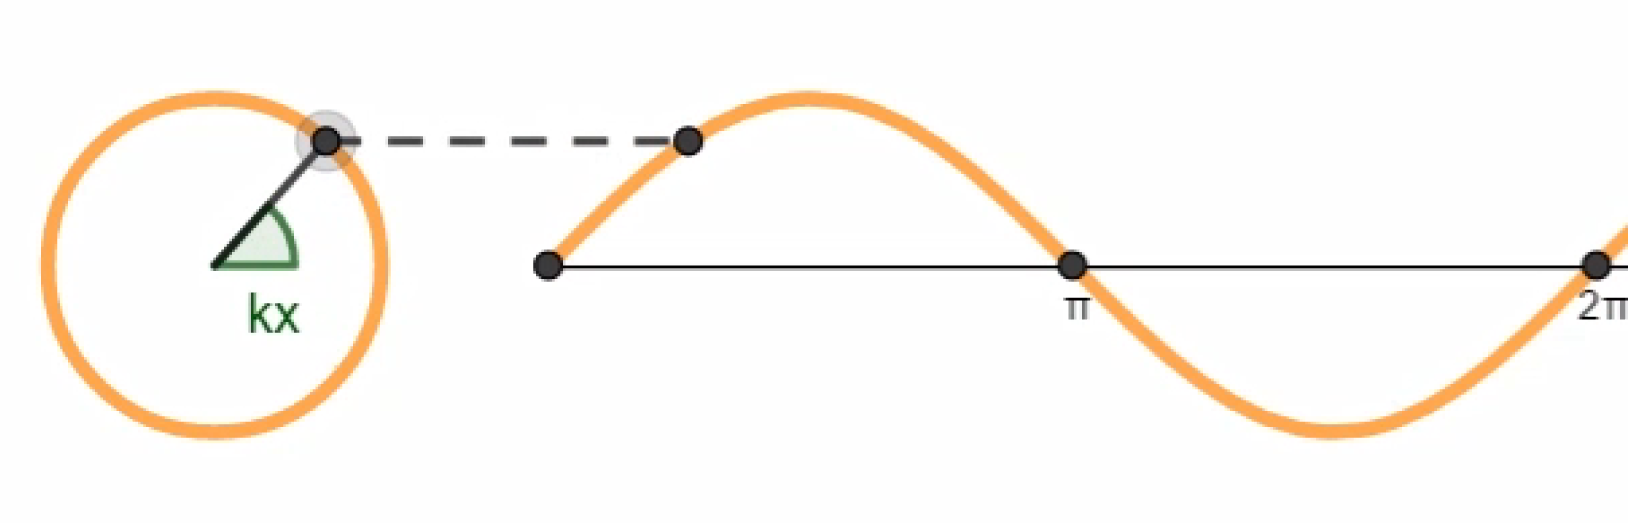
\includegraphics[width=\textwidth, center]{circle-wave.png}
\caption{示意圖,請注意右邊的座標軸是表示$kx$而不是$x$} \vskip 10 pt
\label{fig:circle-wave}
\end{figure}

\subsubsection{與時間有關的偏移函數}
物理學家很貪心,連時間也要討論,不過我們可以使用剛剛討論出的結果來分析與時間有關的偏移函數,我們知道,一段時間可以由無限多個的瞬間來組成,比喻成相片和影片的話大概就是這樣:

與前面類似,我們看只和時間有關的$\sin$函數。
$$ y = \sin (\omega t) $$

同樣,因為波的週期不是$2\pi$,所以要乘上一個數$\omega$,念作omega這裡所指的週期和上面有點不太一樣,上面的是指位置上的周期,而這裡是指時間上的週期,位置上的週期就是你\textbf{某一瞬間看到的(固定時間)}波形走多長會循環一次,而時間的週期就是指對於繩子上\textbf{某一點(固定位置)}時間過多久會回到原點(循環一次),以類似的方法尋找$ω$與$T$的關係。(注意這邊$t$代表時間,是變數;而$T$代表週期,是已經決定於波的常數)

所以對這個函數來說,$\sin$裡面包的是$\omega t$,我們把他當成單位圓上某點的的角度,當$t$逐漸增大,$\omega t$這個相角也開始改變,而且如果我們已知這個波的週期為$T$,所以當$t$從$t_0$慢慢增加到$t_0+T$的時候,$\omega t$也剛好走了一圈($2\pi$),所以會有
$$
\omega\left(t_{0}+T\right)-\omega\left(t_{0}\right)=2 \pi
$$

所以
$$
\omega=\frac{2 \pi}{T}
$$

{\Kai 【想想看,$x_0$,$t_0$的值有什麼意義?】}

\section{波的現象}
\begin{enumerate}
\item \textbf{波的疊加}:當兩個繩波相遇時,兩個波的偏移是可以疊加的,如果一個是高,一個是低,就像是兩側都有人在拉你一樣,會完全消除,如果兩個同為高,或同為低,疊在一起就會變得更高或更低。


\item \textbf{駐波}:如果繩子上有兩個反向但一樣的波,反向的通常是因為波的反射造成的,那麼他就會形成駐波,如下圖所示,任何你所看到的樂器幾乎都是基於駐波的原理。上google搜尋駐波會有很多直觀的動畫。

\begin{figure}[H]
\centering
\graphicspath{{physics/}}
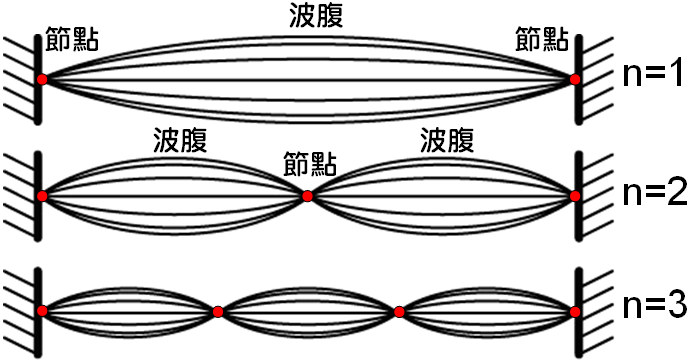
\includegraphics[width=10cm, center]{stationary_wave.png}
\caption{駐波示意圖} \vskip 10 pt
\label{fig:stationary_wave1}
\end{figure}

\begin{figure}[H]
\centering
\graphicspath{{physics/}}
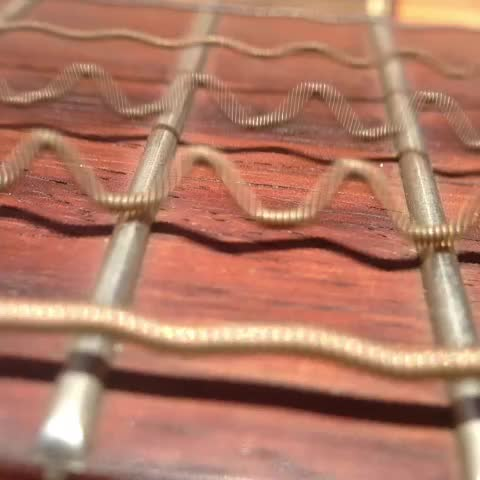
\includegraphics[width=7cm, center]{guitar.jpg}
\caption{吉他彈奏時,會產生駐波(肉眼通常不可見)} \vskip 10 pt
\label{fig:guitar}
\end{figure}

\item \textbf{波的干涉}:假設你有一隻鴨鴨,他在水面上漂浮著,他上下震盪產生週期性的水波向四方散去,現在,假設你有兩隻鴨鴨,假設這兩隻鴨鴨的震盪頻率一樣(即$\omega$一樣),兩隻鴨鴨個別產生的水波將會互相\textbf{干涉}成為下圖的情況。
\begin{figure}[H]
\centering
\graphicspath{{physics/}}
\includegraphics[width=\textwidth, center]{interfere.png}
\label{fig:interfere}
\end{figure}
\end{enumerate}


因為我們很難讓兩隻鴨鴨以完全相同的頻率震動,所以我們通常使用雙狹縫來進行這種干涉,因此這種現象被稱為\textbf{雙狹縫干涉},而且只需要一隻鴨鴨,把鴨鴨產生的水波用一塊板子擋住,並挖兩個很小的洞,則這個水波就會穿越這兩個小洞,產生一樣的現象。而且你可以發現,在打在裡面牆上的強度是條紋分布的,稱為\textbf{干涉條紋}。

為什麼會產生這種干涉條紋呢?因為水面上某一點到兩個波源的距離不同,會導致下列三種不同情況,$S_1$,$S_2$分別表示兩個波源。
\begin{figure}[H]
\centering
\graphicspath{{physics/}}
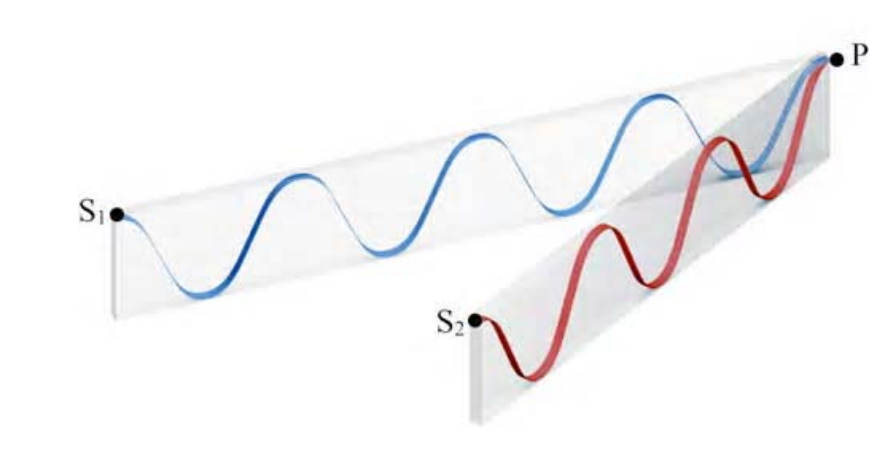
\includegraphics[width=7cm, center]{construct.png}
\caption{兩波峰重疊處,產生建設性干涉,能使其向上的合成位移更大} \vskip 10 pt
\label{fig:con1}
\end{figure}

\begin{figure}[H]
\centering
\graphicspath{{physics/}}
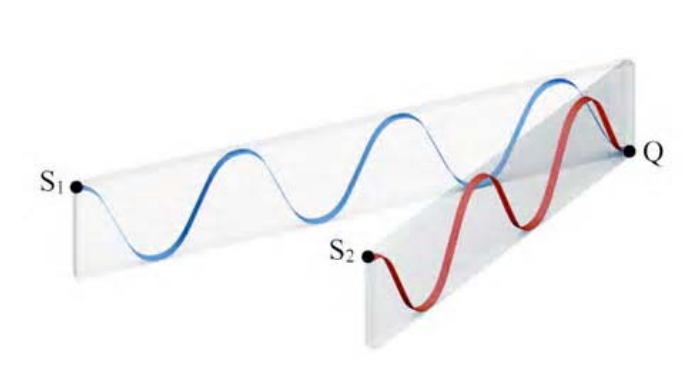
\includegraphics[width=7cm, center]{construct2.png}
\caption{兩波谷重疊處,也產生建設性干涉,能使其向下的合成位移更大} \vskip 10 pt
\label{fig:con2}
\end{figure}

\begin{figure}[H]
\centering
\graphicspath{{physics/}}
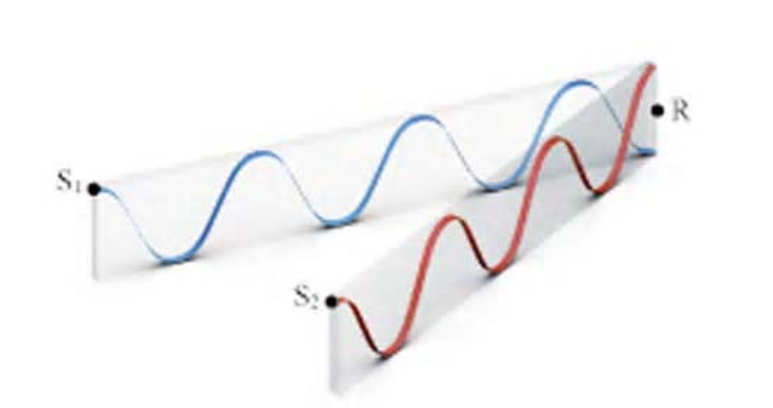
\includegraphics[width=7cm, center]{destruct.png}
\caption{波峰與波谷重疊處,產生破壞性干涉,能使其合成位移為零} \vskip 10 pt
\label{fig:de}
\end{figure}

{\Kai 【想想看,這三種情況會發生在上面那張水波圖的那些位置?(淺色的代表波峰、深色則代表波谷)】}





\section{附錄:利用坐標轉換概念推導偏移函數}


我們知道一個靜止的正弦波長這樣:$\sin⁡ \left (kx\right )$
若要讓他開始運動,則$x$的形式必須改變。

首先,想像這個波開始運行,但是杰穎站在這個波上,隨著這個波前進,設波速為$v$向著$x$軸正向運動,那麼這個人的速度也必定為$v$,杰穎因為什麼都有,所以他也有個以自己為圓點的坐標系$(x^{\prime}, y^{\prime})$,這個「$\prime$」表示他和站在地面上原本的靜止坐標系$(x,y)$是不同的坐標系。對於這個移動中的杰穎來說,因為他和波沒有相對運動,所以他看到的波是靜止的,他用他自己的坐標系描述的話就是
$$
y^{\prime}=\sin \left(\frac{2 \pi}{\lambda} x^{\prime}\right)
$$

因為$(x^{\prime}, y^{\prime})$這個坐標系相對於$(x,y)$往$x$軸正向進行運動,假設兩個在$t=0$的時候重合,那麼兩個坐標系之間就會滿足
$$
\begin{array}{c}{y=y^{\prime}} \\ {x^{\prime}=x-v t}\end{array}
$$
將杰穎坐標系轉換回地面的靜止坐標系,且使用$\frac{v}{\lambda}=\frac{1}{T}$
$$
y^{\prime}=\sin \left(\frac{2 \pi}{\lambda} x^{\prime}\right) \Rightarrow y=\sin \left[\frac{2 \pi}{\lambda}(x-v t)\right]=\sin \left(\frac{2 \pi}{\lambda} x-\frac{2 \pi}{\lambda} v t\right)=\sin \left(\frac{2 \pi}{\lambda} x-\frac{2 \pi}{T} t\right)
$$

定義$\frac{2\pi}{\lambda}\equiv k$ (波數)、$\frac{2\pi}{T} \equiv \omega$ (角速度),可以把公式整理成
$$
y=\sin (k x-\omega t)
$$

如果原始波函數為零的地方不在原點上,多一段距離則相當多一個相位角 $\phi_0$,則變為
$$
y=\sin \left(k x-\omega t+\phi_{0}\right)
$$

這個就稱為移動後的正弦波函數。
